\documentclass[12pt,letterpaper]{article}
\usepackage{graphicx}
\usepackage{amssymb}
\usepackage{amsmath}
\usepackage{alltt}
\usepackage{listings}
\usepackage{natbib}
\bibpunct{(}{)}{;}{a}{}{,}
\usepackage[pdftex,colorlinks,bookmarks,citecolor=blue,%
  bookmarksnumbered,bookmarksopen=true,breaklinks,%
  hyperfootnotes=false]{hyperref}
\usepackage[width=6.5in,height=9in]{geometry}
\usepackage{setspace}

\newcommand\micron{\mbox{$\mu$m}}%
\newcommand\arcdeg{\mbox{$^\circ$}}%
\newcommand\arcmin{\mbox{$^\prime$}}%
\newcommand\arcsec{\mbox{$^{\prime\prime}$}}%
\newcommand\phm[1]{\phantom{#1}}%
\newcommand\nodata{ ~$\cdots$~ }%
\newcommand\inv{$^{-1}$}
\newcommand\mjysr{MJy~sr$^{-1}$}
\newcommand\invrho{~$\rho^{-1}$}
\newcommand\kms{km~s$^{-1}$}
\newcommand\wcm{W~cm$^{-2}$~\micron$^{-1}$}
\newcommand\gcm{g~cm$^{-3}$}
\newcommand\mks{J~K$^{-1}$~m$^{-2}$~s$^{-1/2}$}
\newcommand\degr{\arcdeg}%
\newcommand\Sun{\sun}% Sun symbol, "S"
\newcommand\sun{\odot}%
\newcommand\sst{\textit{Spitzer Space Telescope}}
\newcommand\spitzer{\textit{Spitzer}}
\newcommand\iso{\textit{ISO}}
\newcommand\isolong{\textit{Infrared Space Observatory}}
\newcommand\rundynamics{RunDynamics}
\newcommand\cs{CometSuite}
\newcommand\bvec[1]{\boldsymbol{#1}}


\begin{document}
\title{CometSuite}
\author{Michael S. Kelley\\
Department of Astronomy\\
University of Maryland, College Park\\
{\small msk @t astro.umd.edu}}

\date{30 Mar 2009}
\maketitle
\tableofcontents

\clearpage

\section{Introduction}
\cs{} is a set of C/C++ and IDL programs primarily designed for
modeling and analysing comet dust dynamics.  The \cs{}:~IDL programs
are used to determine comet, planet, and \spitzer{} positions in the
solar system; and to compute comet ephemerides for an arbitrary
observer.  The \cs{}:~\rundynamics{} programs simulate comet dust
dynamics; create syndyne files suitable for use in SAOImage/DS9;
create projected images of a comet simulation; and to inspect and
verify \rundynamics{} data files.  Below, \S\ref{sec:cs-install}
describes the installation of the \cs{}, \S\ref{sec:cs-idl} presents
the IDL programs, and \S\ref{sec:cs-rd} presents the \rundynamics{}
programs.

%%%%%%%%%%%%%%%%%%%%%%%%%%%%%%%%%%%%%%%%%%%%%%%%%%%%%%%%%%%%%%%%%%%%%%%%%%%%%%%%
% installation
%%%%%%%%%%%%%%%%%%%%%%%%%%%%%%%%%%%%%%%%%%%%%%%%%%%%%%%%%%%%%%%%%%%%%%%%%%%%%%%%
\section{CometSuite: Installation}\label{sec:cs-install}

\lstset{language=csh,basicstyle=\normalsize\ttfamily\singlespacing,
  showstringspaces=false,columns=fullflexible}

\subsection{Requirements}
Below is a list of the required files.  All but the IDL Astro programs
will be explained.  The \cs{} has been successfully installed on
GNU/Linux and Solaris workstations.  For Solaris installations, the
\cs{} should be compiled for 64-bit mode.  GNU/Linux installation can
be either 32-bit or 64-bit, depending on the system's native
architecture.  Compiling in 64-bit mode facilitates a smooth
interaction with 64-bit IDL.

\begin{itemize}
\item IDL Astro programs: \url{http://idlastro.gsfc.nasa.gov/}.

\item The CCfits and Cfitsio libraries, C/C++ interfaces to create
FITS files.

\item The CSPICE Toolkit from NASA/JPL's Navigation and Ancillary
Information Facility (NAIF).  CSPICE is a library interface to NAIF
ephemeris files.  This library returns the location of planets,
spacecraft, comets, or whatever object we have loaded in a SPICE
kernel.

\item Ephemeris files for the planets and the \textit{Spitzer Space
Telescope}.

\item Comet ephemeris files.  You can generate these with the JPL
HORIZONS program via a telnet interface.

\end{itemize}

\subsection{Installation}\label{sec:install}
\subsubsection{Extract}
First, extract the tarball into a permanent directory.  Here, the
\cs{} is located in \texttt{\$HOME/Projects}.
\begin{lstlisting}
cd ~/Projects
tar xzvf cometsuite.tar.gz
\end{lstlisting}
The following directory structure will be created and filled with files.
\begin{lstlisting}
cometsuite
cometsuite/bin
cometsuite/doc
cometsuite/doc/articles
cometsuite/idl
cometsuite/idl/astrometry
cometsuite/idl/graphics
cometsuite/idl/misc
cometsuite/idl/tools
cometsuite/include
cometsuite/kernels
cometsuite/kernels/getkerns
cometsuite/lib
cometsuite/src
cometsuite/src/getxyz
cometsuite/src/rundynamics-0.6
cometsuite/src/rundynamics-0.6/bin
cometsuite/src/rundynamics-0.6/doc
cometsuite/src/rundynamics-0.6/include
cometsuite/src/rundynamics-0.6/src
cometsuite/src/rundynamics-0.6/test
cometsuite/src/rundynamics-0.6/test/scripts
cometsuite/src/rundynamics-0.7
cometsuite/src/rundynamics-0.7/bin
cometsuite/src/rundynamics-0.7/doc
cometsuite/src/rundynamics-0.7/include
cometsuite/src/rundynamics-0.7/src
cometsuite/src/rundynamics-0.7/test
cometsuite/src/rundynamics-0.7/test/scripts
cometsuite/src/userguide
\end{lstlisting}

\subsubsection{Cfitsio and CCfits}

Cfitsio and CCfits are not included in the \cs{} package.  You may
already have these installed on your system, in which case you could
skip this section\footnote{If the Cfitsio and CCfits libraries are
  installed to a non-standard location (i.e., not the \cs{} directory
  and not /usr, /usr/local, etc.), be sure to include the directories in
  the \texttt{LD\_LIBRARY\_PATH} and \texttt{CPATH} environment
  variables.}.  The programs can also be automatically compiled and
installed within the cometsuite directory, which is the recommended
method.

Download Cfitsio\footnote{\url{http://heasarc.gsfc.nasa.gov/fitsio/}}
and extract into the \cs{} \texttt{./src} directory.
\begin{lstlisting}
cd ~/Projects/cometsuite/src
tar xzvf /path/to/cfitsio3006.tar.gz
\end{lstlisting}

Download the CCfits
library\footnote{\url{http://heasarc.nasa.gov/fitsio/CCfits/}} and extract.
\begin{lstlisting}
cd ~/Projects/cometsuite/src
tar xzvf /path/to/CCfits-1.5.tar.gz
\end{lstlisting}

\subsubsection{NAIF CSPICE}
The CSPICE toolkit contains some useful tools that will be copied to
the \cs{} bin directory.  The program \texttt{brief} gives a quick
description of a SPICE kernel, and is the most commonly used tool.
For the curious, the tools are documented in the \texttt{cspice/doc}
directory.

Download the GCC version of the CSPICE
toolkit\footnote{\url{ftp://naif.jpl.nasa.gov/pub/naif/toolkit/C/Sun_Solaris_GCC_64bit/packages/cspice.tar.Z}
for Solaris,
\url{ftp://naif.jpl.nasa.gov/pub/naif/toolkit/C/PC_Linux_GCC_32bit/packages/cspice.tar.Z},
for 32-bit GNU/Linux, and
\url{ftp://naif.jpl.nasa.gov/pub/naif/toolkit/C/PC_Linux_GCC_64bit/packages/cspice.tar.Z}
for 64-bit GNU/Linux}.  Extract the files to the \cs{} \texttt{./src}
directory.
\begin{lstlisting}
cd ~/Projects/cometsuite/src
tar xzvf /path/to/cspice.tar.Z
\end{lstlisting}

CSPICE should compile automatically with the \cs{} Makefile.  The rest
of this section may be skipped.

On 64-bit machines, CSPICE must be compiled with the -fPIC and -m64
options enabled via the following line:
\begin{lstlisting}
setenv TKCOMPILEOPTIONS "-c -m64 -ansi -O2 -DNON_UNIX_STDIO -fPIC"
\end{lstlisting}
All users compile and install CSPICE as follows.
\begin{lstlisting}
cd cspice
csh makeall.csh
cp exe/* ../../bin
cp lib/* ../../lib
cp include/Spice*.h ../../include
\end{lstlisting}

\subsubsection{SPICE Kernels}
Kernels contain the states (position, velocity, orientation) of solar
system bodies and spacecraft.  Place all your kernels in the
\texttt{./cometsuite/kernels} directory.

First, download the planetary constants and leap-seconds
kernels\footnote{\url{ftp://naif.jpl.nasa.gov/pub/naif/generic_kernels/pck/pck00008.tpc}
  and
  \url{ftp://naif.jpl.nasa.gov/pub/naif/generic_kernels/lsk/naif0009.tls}}.
The current leap second kernel is version 9, which includes the 31
December 2008 leap-second, but your mileage may vary.  Next, download
a planetary ephemeris
file.\footnote{\url{ftp://ssd.jpl.nasa.gov/pub/eph/planets/bsp/}} I
have been using JPL's DE-414 with good results \citep{standish06}, but
the current standard is DE-421 \citep{folkner08}.  Finally, get the
latest \sst{} kernel.\footnote{For example, the file
  spk\_030825\_050815\_091231.bsp at
  \url{ftp://naif.jpl.nasa.gov/pub/naif/SIRTF/kernels/spk/}, where
  030825 is the launch date, 050815 is the file creation date, and
  091231 is the date of the last calculated position.}

\subsubsection{HORIZONS Kernels}
The positions of other solar system bodies, such as comets, are
calculated by JPL's HORIZONS ephemeris generator.  Obtain asteroid and
comet kernels as follows:
\begin{enumerate}
\item Connect to HORIZONS via the telnet interface:\\ \texttt{telnet
ssd.jpl.nasa.gov 6775}

\item Select body 2P/Encke (case sensitive):\\ \texttt{Horizons> 2P}

\item At the time of writing, Encke has over 50 orbital solutions,
spanning from 1786 to the present.  We need to select the most recent
orbit.  The record number is 900088 for the 2005 orbital elements, but
JPL/SSD reserves the right to change the record number at any time,
\texttt{Select ... [F]tp, [M]ail, [R]edisplay, ?, <cr>: 900088}

\item Generate a [S]PK file (SPICE kernel):\\ \texttt{Select
... [A]pproaches, [E]phemeris, [F]tp,[M]ail,[R]edisplay,}\\\texttt{ [S]PK,?,<cr>:
s }

\item HORIZONS asks for you e-mail address:\\ \texttt{Enter your
Internet e-mail address [?]: msk@astro.umn.edu}

\item I always use the binary format, but some machines are
incompatible with HORIZONS's binary files.  In that case, use the text
format and convert the file after the download with the SPICE toolkit
program \texttt{tobin}:\\ \texttt{SPK text transfer format [ YES, NO,
? ] : n}

\item Enter the dates you would like HORIZONS to calculate the
ephemeris, \rundynamics{} will not be able to integrate particles
outside of these limits.  I typically use 1980--2010, although,
technically, the orbit solution (900088) we selected isn't valid for
such a large range in time (hence all the orbit solutions listed
above):\\ \texttt{SPK object START [ t >= 1900-Jan-01, ?  ] :
1980-1-1\\SPK object STOP [ t <= 2101-Jan-01, ? ] : 2010-1-1}

\item Your SPK file is created.  I suggest one comet per file:\\
\texttt{Add more objects to file  [ YES, NO, ? ] : n}

\item Retrieve the file and store in your
\texttt{./cometsuite/kernels} directory:\\
\texttt{You have 30 minutes to retrieve the following by anonymous FTP:\\
  Machine name:  ssd.jpl.nasa.gov\\
  Directory   :  cd to "/pub/ssd/"\\
  File name   :  wld6263.15\\
  File type   :  BINARY   $>$* set FTP binary mode *$<$\\
  Full path   :  ftp://ssd.jpl.nasa.gov/pub/ssd/wld6263.15\\
\\
Select ... [E]phemeris, [M]ail, [R]edisplay, ?, <cr>: q\\
\$ wget ftp://ssd.jpl.nasa.gov/pub/ssd/wld6263.15}

\item A note on kernel file names. For ease of use with the \cs{}
IDL programs, save the kernel file using the name of the comet in
lower-case and spaces and punctuation removed. For example, the
default kernel file for a comet named ``Wild 2'' is wild2.bsp, or for
``Churyumov-Gerasimenko'', churyumovgerasimenko.bsp.
\end{enumerate}

\subsubsection{Compilation}
Edit the top-level make file (\texttt{./cometsuite/Makefile}) and set
the kernel variables to the appropriate values.  Also make sure the
MARCH variable is set to -m64 for 64-bit machines, -m32 for everything
else.  Now run the make file, omitting cfitsio and ccfits if these are
already installed elsewhere:
\begin{lstlisting}
cd ~/Projects/cometsuite
make depclean cfitsio ccfits all
\end{lstlisting}
The Makefile will compile and install CSPICE, Cfitsio, CCfits, and
\rundynamics{} to the \cs{} directory.  The depclean option to Make
cleans the pre-compiled CSPICE library (the pre-built library can
cause problems during \cs{} building).

Finally, add the \cs{} binary directory to your PATH environment
variable and the \cs{} idl directory to your IDL\_PATH environment
variable, e.g.:
\begin{lstlisting}
setenv IDL_PATH ${IDL_PATH}:+~/Projects/cometsuite/idl
setenv PATH ${PATH}:~/Projects/cometsuite/bin
\end{lstlisting}
The \cs{} is ready to go.

\subsubsection{Program Checkout}
Test your \cs{} installation in IDL.  Get the heliocentric
positions of the planets on 01~Jan~2006.
\begin{lstlisting}
get_planet_xyz,julday(01,01,2006,0d),511d,r
print,r[*,2]
      -26412201.   1.4471277e+08      -1906.9767
\end{lstlisting}
The vector r[*,2] is the x, y, z position of the Earth-Moon barycenter
in kilometers.

Once you have a comet ephemeris kernel you can get the position of a
comet in the sky.  For example, comet Encke as observed by Earth and
\textit{Spitzer} on 23~Jun~2004.
\begin{lstlisting}
IDL> comet_astrom,'encke',[2004,6,23]

                           Comet: encke
                            Date: 2004-06-23
                   Time (UT hrs):  0.00000
                      Julian day: 2453179.50000

      Heliocentric distance (AU):    2.554
        Geocentric distance (AU):    1.937
   Spitzer-centric distance (AU):    1.999

     Sun-Comet-Earth angle (deg):   20.912
   Sun-Comet-Spitzer angle (deg):   21.699

                   Earth RA, Dec: 22:37:15.9  -14:31:20.5
                 Spitzer RA, Dec: 22:39:25.0  -13:39:39.7

       Earth projected sun (deg):   70.717
  Earth projected velocity (deg):   32.616
     Spitzer projected sun (deg):   68.974
Spitzer projected velocity (deg):   32.592
\end{lstlisting}
Now, correct the ephemeris for light travel time with the
\texttt{/ltt} option.
\begin{lstlisting}
IDL> comet_astrom,'encke',[2004,6,23],/ltt
CometSuite directory found: /home/msk/Projects/cometsuite/idl/../
Kernel directory set to: /home/msk/Projects/cometsuite/idl/../kernels/

                           Comet: encke
                            Date: 2004-06-23
                   Time (UT hrs):  0.00000
                      Julian day: 2453179.50000

      Heliocentric distance (AU):    2.554
        Geocentric distance (AU):    1.937
   Spitzer-centric distance (AU):    1.999

     Sun-Comet-Earth angle (deg):   20.915
   Sun-Comet-Spitzer angle (deg):   21.702

                   Earth RA, Dec: 22:37:16.2  -14:31:17.9
                 Spitzer RA, Dec: 22:39:25.3  -13:39:37.3
                                  (light travel corrected)

       Earth projected sun (deg):   70.716
  Earth projected velocity (deg):   32.609
     Spitzer projected sun (deg):   68.973
Spitzer projected velocity (deg):   32.585
\end{lstlisting}

Test the \rundynamics{} programs.  Before you run the \rundynamics{}
test suite, download the SPICE kernels for 2P/Encke, 28P/Neujmin,
29P/Schwassmann-Wachmann, and 67P/Churyumov-Gerasimenko (saved as
files encke.bsp, neujmin1.bsp, schwassmannwachmann1.bsp,
churyumovgerasimenko.bsp).  You will also need gnuplot.\footnote{Not
  really, but the Makefile will try and plot the results with gnuplot
  when the tests are completed} Run the test suite with the provided
Makefile.
\begin{lstlisting}
cd ~/Projects/cometsuite
make test
\end{lstlisting}

The first test creates a set of syndynes and verifies the output file
can be written properly (the average $\beta$ should not differ from
below).
\begin{lstlisting}
../bin/rundynamics syntest.par
...
../bin/xyzinfo syntest.xyz
...
Average beta: 0.0187143
Successfully read 217 out of 217 particles
\end{lstlisting}

The second test is a Monte-Carlo simulation of a comet coma.  The
average $\beta$ will vary.
\begin{lstlisting}
../bin/rundynamics mctest.par
...
../bin/xyzinfo mctest.xyz
...
Average beta: 0.00634739
Successfully read 100 out of 100 particles
\end{lstlisting}

The third test checks the particle size distribution of the
Monte-Carlo simulation using a bin size of 10~mm.  This should be
$dn/da \propto a^{-1}$, but keep in mind there were only 100 particles
used in the simulation.  $\beta$ is picked from the range
$10^{-6}$--$10^{-1}$.  The result will be shown with Gnuplot after
completion of all remaining tests.
\begin{lstlisting}
../bin/xyz2psd mctest.xyz -o mctest.psd --aper=-1 -b 10000
\end{lstlisting}

The fourth and fifth tests are checks on the accuracy of the
integrator using comets 29P/Schwassman-Wachmann (a nearly circular
orbit) and Neujmin (with an eccentricity of 0.78), respectively.
\rundynamics{} integrates $\beta = 0$ particles over a time span of 20
years.  These comets have no known non-gravitational accelerations and
each $\beta = 0$ particle should reproduce the position of the comet
at the end of the integration.
\begin{lstlisting}
../bin/rundynamics accutest1.par
...
Average beta: 0
Successfully read 21 out of 21 particles

../bin/rundynamics accutest2.par
...
Average beta: 0
Successfully read 21 out of 21 particles

./accutest
...
schwassmann-wachmann 1
age(yr) delta_r(km) delta_v(km/s)
...
output written to accutest1.dat
neujmin 1
particle age(yr) delta_r(km) delta_v(km/s)
...
output written to accutest2.dat
\end{lstlisting}

When the test routines complete, Gnuplot is opened and automatically
presents the results from the Monte-Carlo particle size distribution
test (Fig.~\ref{fig:rd-psdtest}) and the two accuracy tests
(Fig.~\ref{fig:rd-accutest}).  The particle size distribution plot
shows a theoretical trend line and the calculated particle size
distribution from the entire simulation.  \rundynamics{} runs all
simulations with a particle size distribution of $dn/d\log\beta
\propto \beta^{-1}$ to ensure each particle size bin is accurately
represented in the final simulation (see \S\ref{sec:dynamics} for a
discussion).  The accuracy plots show the differences between the test
particles and their parent nucleus.  Most particles have errors less
than 100~km.  The oldest comet Neujmin particles show a trend of
increasing error at the oldest ages.  The integrator has some
difficulty with perihelion passages in orbits of high eccentricity
(comet Neujmin's $P=18$~yr and $e=0.78$).  The
29P/Schwassmann-Wachmann ($P = 15$~yr, $e=0.04$) particles remain at
low errors after perihelion passage ($t\approx15$~yr).  To exit
Gnuplot type \texttt{quit}.  You can redisplay these plots at any
time:
\begin{lstlisting}
cd ~/Projects/cometsuite/dynamics/rundynamics/test
make plots
\end{lstlisting}


%%%%%%%%%%%%%%%%%%%%%%%%%%%%%%%%%%%%%%%%%%%%%%%%%%%%%%%%%%%%%%%%%%%%%%%%%%%%%%%%
% psdtest
%%%%%%%%%%%%%%%%%%%%%%%%%%%%%%%%%%%%%%%%%%%%%%%%%%%%%%%%%%%%%%%%%%%%%%%%%%%%%%%%
\begin{figure}
\center
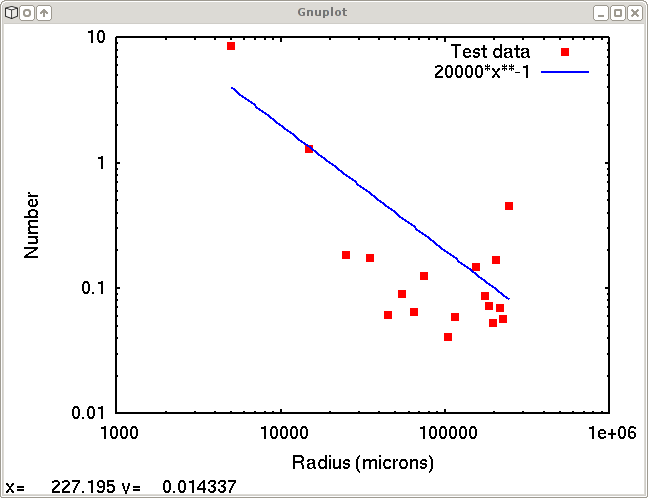
\includegraphics[width=0.5\textwidth]{figures/rd-psdtest}
\caption[The particle size distribution of a \rundynamics{} Monte-Carlo
test.]{The particle size distribution of a \rundynamics{} Monte-Carlo
test.  A successful test is indicated when the theoretical trend line
roughly approximates the data points, as
shown. \label{fig:rd-psdtest}}
\end{figure}
%%%%%%%%%%%%%%%%%%%%%%%%%%%%%%%%%%%%%%%%%%%%%%%%%%%%%%%%%%%%%%%%%%%%%%%%%%%%%%%%

%%%%%%%%%%%%%%%%%%%%%%%%%%%%%%%%%%%%%%%%%%%%%%%%%%%%%%%%%%%%%%%%%%%%%%%%%%%%%%%%
% accutest
%%%%%%%%%%%%%%%%%%%%%%%%%%%%%%%%%%%%%%%%%%%%%%%%%%%%%%%%%%%%%%%%%%%%%%%%%%%%%%%%
\begin{figure}
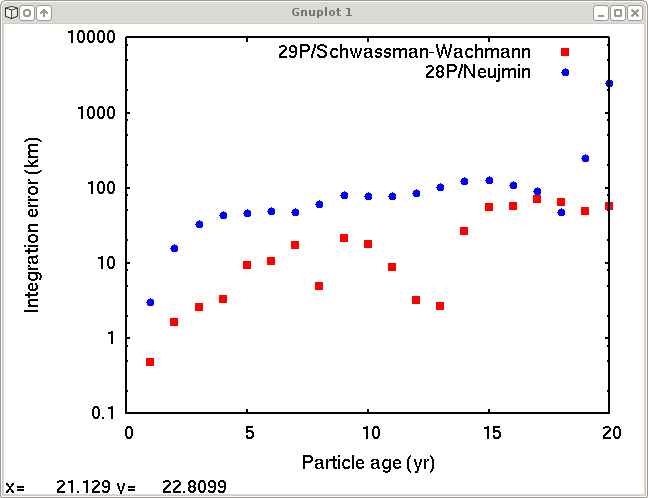
\includegraphics[width=0.5\textwidth]{figures/rd-accutest1}
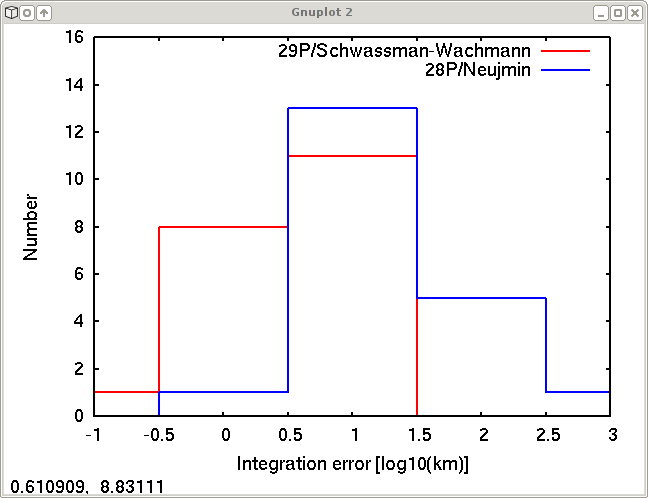
\includegraphics[width=0.5\textwidth]{figures/rd-accutest2}
\caption[Results from a \rundynamics{} accuracy test.]{Results from a
\rundynamics{} accuracy test. \label{fig:rd-accutest}}
\end{figure}
%%%%%%%%%%%%%%%%%%%%%%%%%%%%%%%%%%%%%%%%%%%%%%%%%%%%%%%%%%%%%%%%%%%%%%%%%%%%%%%%

\subsection{A Note About Command Line Parameters}

Take care when typing command line parameters.  Keep in mind the
following examples are equivalent,
\begin{itemize}
\item \texttt{xyz2fits -a -5.8 ...}
\item \texttt{xyz2fits -a-5.8 ...}
\item \texttt{xyz2fits -a "-5.8" ...}
\item \texttt{xyz2fits -a "-5.8" ...}
\end{itemize}
or, if the parameter allows, use the long option,
\begin{itemize}
\item \texttt{xyz2fits --afrho=-5.8 ...}
\item \texttt{xyz2fits --afrho -5.8 ...}
\end{itemize}
But the examples below are \textbf{invalid} inputs,
\begin{itemize}
\item \texttt{xyz2fits -a=-5.8 ...}
\item \texttt{xyz2fits --afrho-5.8 ...}
\end{itemize}

\subsection{The Dynamical Modeler and Visualizations}
The dynamical modeler is a C/C++ program designed to simulate comet
dust dynamics.  Begin exploring \rundynamics{} and generate an example
parameter file:
\begin{lstlisting}
msk@ccec]: rundynamics -e > syndynes.par
msk@ccec]: cat syndynes.par
# valid program names: syndynes, make comet
PROGRAM: Syndynes
# parameters common to all programs
COMET: encke
KERNEL: encke.bsp
JD: 2450643.54170
XYZFILE: iso_observation.xyz
PFUNC: 
TOL: 1e-2
PLANETS: 511
PLANETLOOKUP: off
CLOSEAPPROACHES: on
LTT: no
# syndyne specific section
BETA: 1e-3 2e-3 4e-3 6e-3 8e-3 1e-2 1e-1
NDAYS: 200
STEPS: 31
ORBIT: 1
# mccomet specific section
NPARTICLES: 
\end{lstlisting}
You can get a detailed description of each parameter using the long
option \texttt{--example}.

\subsection{Syndynes}\label{sec:rd-example}
Run the following example to create syndynes for comet 2P/Encke at the
time of the \citet{reach00} observation with the \isolong{} in
July~1997:
\begin{lstlisting}
cat >encke.par<<EOF
PROGRAM: Syndynes
COMET: encke
KERNEL: encke.bsp
JD: 2450643.54170
XYZFILE: iso_observation.xyz
TOL: 1e-2
PLANETS: 511
PLANETLOOKUP: off
CLOSEAPPROACHES: on
LTT: no
BETA: 1e-3 2e-3 4e-3 6e-3 8e-3 1e-2 1e-1
NDAYS: 200
STEPS: 31
ORBIT: 1
EOF
rundynamics encke.par
\end{lstlisting}
When the simulation completes, run IDL and plot the data.
\begin{lstlisting}
synplot,'iso_observation.xyz',[60,-60],[-60,60],/arcmin,/color
\end{lstlisting}
The resultant plot is presented in Fig.~\ref{fig:rd-syndynes}.

%%%%%%%%%%%%%%%%%%%%%%%%%%%%%%%%%%%%%%%%%%%%%%%%%%%%%%%%%%%%%%%%%%%%%%%%%%%%%%%%
% syndynes
%%%%%%%%%%%%%%%%%%%%%%%%%%%%%%%%%%%%%%%%%%%%%%%%%%%%%%%%%%%%%%%%%%%%%%%%%%%%%%%%
\begin{figure}
\center
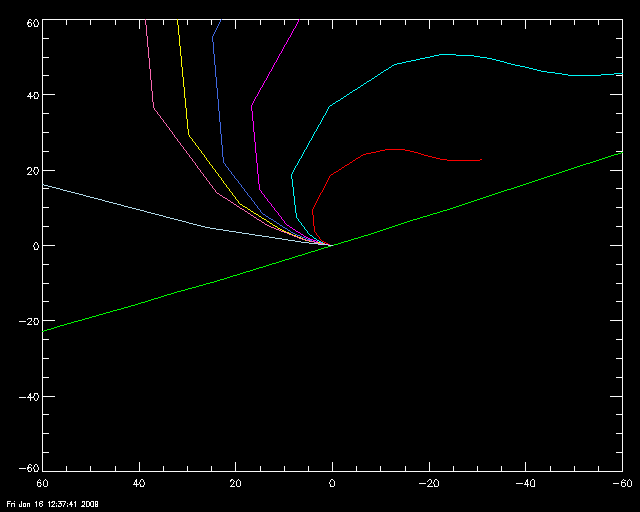
\includegraphics[width=0.5\textwidth]{figures/rd-syndynes}
\caption{Comet 2P/Encke syndynes calculated and plot by the
\cs{}. \label{fig:rd-syndynes}}
\end{figure}
%%%%%%%%%%%%%%%%%%%%%%%%%%%%%%%%%%%%%%%%%%%%%%%%%%%%%%%%%%%%%%%%%%%%%%%%%%%%%%%%

We may also use SAOImage/DS9 to plot the syndynes.  First, convert the
syndynes into a DS9 regions file, then open the ISO observation and
regions.  In the following example, the observer is Earth, but
\spitzer{} is also a valid option provided the observation occurred
during \textit{Spitzer}'s lifetime.
\begin{lstlisting}
syn2ds9 --observer=earth -o iso_observation.reg iso_observation.xyz
ds9 -scale log -scale limits 0 500 encke_shift.fits \
  -regions iso_observation.reg
\end{lstlisting}
The results are shown in Fig.~\ref{fig:rd-ds9}.  There appears to be a
small shift in the projection.  The Julian date may be slightly off in
the syndyne parameter file.  An other possibility is that the syndynes
should have been calculated with Encke's orbital elements from 1997.
The offset may be remedied with the offset option to \texttt{syn2ds9}.
\begin{lstlisting}
syn2ds9 --observer=earth -o iso_observation.reg  --offset=-997,-12 \
  iso_observation.xyz
\end{lstlisting}

%%%%%%%%%%%%%%%%%%%%%%%%%%%%%%%%%%%%%%%%%%%%%%%%%%%%%%%%%%%%%%%%%%%%%%%%%%%%%%%%
% ds9
%%%%%%%%%%%%%%%%%%%%%%%%%%%%%%%%%%%%%%%%%%%%%%%%%%%%%%%%%%%%%%%%%%%%%%%%%%%%%%%%
\begin{figure}
\center
%\includegraphics[width=0.5\textwidth]{figures/rd-ds9}
\caption{Comet 2P/Encke syndynes calculated and plot by the
\cs{}, displayed in SAOImage/DS9. \label{fig:rd-ds9}}
\end{figure}
%%%%%%%%%%%%%%%%%%%%%%%%%%%%%%%%%%%%%%%%%%%%%%%%%%%%%%%%%%%%%%%%%%%%%%%%%%%%%%%%


\subsection{The SPICE Tool \texttt{brief}}
The SPICE program \texttt{brief} summarizes SPICE kernels (a more
detailed inspection is obtained with \texttt{spacit}).
\begin{lstlisting}
msk@ccec]: brief de405.bsp 
Brief.  Version: 2.2.0        (SPICE Toolkit N0058)
 
 
Summary for: de405.bsp
 
Bodies: MERCURY BARYCENTER (1)  SATURN BARYCENTER (6)   MERCURY (199)
        VENUS BARYCENTER (2)    URANUS BARYCENTER (7)   VENUS (299)
        EARTH BARYCENTER (3)    NEPTUNE BARYCENTER (8)  MOON (301)
        MARS BARYCENTER (4)     PLUTO BARYCENTER (9)    EARTH (399)
        JUPITER BARYCENTER (5)  SUN (10)                MARS (499)
        Start of Interval (ET)              End of Interval (ET)
        --------------------------------    --------------------------------
        1599 DEC 09 00:00:00.000            2201 FEB 20 00:00:00.000
 
msk@ccec]: brief churyumovgerasimenko.bsp 
Brief.  Version: 2.2.0        (SPICE Toolkit N0058)
 
 
Summary for: churyumovgerasimenko.bsp
 
Body: CHURYUMOV-GERASIMENKO (1000012)
      Start of Interval (ET)              End of Interval (ET)
      --------------------------------    --------------------------------
      1980 JAN 01 00:00:00.000            2010 JAN 01 00:00:00.000

msk@ccec]: brief schwassmannwachmann3.bsp
Brief.  Version: 2.2.0        (SPICE Toolkit N0058)
 
 
Summary for: schwassmannwachmann3.bsp
 
Body: 1000394
      Start of Interval (ET)              End of Interval (ET)
      --------------------------------    --------------------------------
      1980 JAN 01 00:00:00.000            2010 JAN 01 00:00:00.000
\end{lstlisting}
Notice that the kernel for comet 29P/Schwassmann-Wachmann does not
list the name of the comet, only the NAIF ID is shown (1000394), but
the 67P/Churyumov-Gerasimenko kernel lists that comet's name.  When a
kernel does not contain the comet name, it must be referenced by NAIF
ID in all \cs{} programs.  Always check new kernel files before using
them.
\begin{lstlisting}
IDL> comet_astrom,'1000394',[2006,5,15],kernel='schwassmannwachmann3.bsp'
CometSuite directory found: /home/msk/Projects/cometsuite/idl/../
Kernel directory set to: /home/msk/Projects/cometsuite/idl/../kernels/

                           Comet: 1000394
                            Date: 2006-05-15
                   Time (UT hrs):  0.00000
                      Julian day: 2453870.50000

      Heliocentric distance (AU):    0.996
        Geocentric distance (AU):    0.087
   Spitzer-centric distance (AU):    0.397

     Sun-Comet-Earth angle (deg):   97.200
   Sun-Comet-Spitzer angle (deg):   80.363

                   Earth RA, Dec: 21:55:25.4   17:07:45.5
                 Spitzer RA, Dec: 21:14:15.6  -06:52:16.6

       Earth projected sun (deg):   73.937
  Earth projected velocity (deg):  152.902
     Spitzer projected sun (deg):   73.330
Spitzer projected velocity (deg):  115.068
\end{lstlisting}
Alternatively, you can create a link to the schwassmannwachmann3.bsp
file named 1000394.bsp and drop the kernel option altogether.
\begin{lstlisting}
cd ~/Projects/cometsuite/kernels
ln -s schwassmannwachmann3.bsp 1000394.bsp
idl
comet_astrom,'1000394',[2006,5,15]
\end{lstlisting}

%%%%%%%%%%%%%%%%%%%%%%%%%%%%%%%%%%%%%%%%%%%%%%%%%%%%%%%%%%%%%%%%%%%%%%
\begin{thebibliography}{}
\bibitem[Standish(2006)]{standish06} Standish, E.~M.\ 2006,
JPL IOM, 343.R-06-002

\bibitem[Folkner et al.(2008)]{folkner08} Folkner, W.~M., Williams,
  J.~G., \& Boggs, D.~H.\ 2008, JPL IOM, 343R-08-003

\end{thebibliography}

\end{document}
